\section{IDENTIFICACIÓN DE LOS COMPONENTES DE UNA LÍNEA DE TRANSMISIÓN ELÉCTRICA EN EL ÁREA METROPOLITANA DE BUCARAMANGA}

La torre de transmisión analizada (\figurename~\ref{fig:Torre} y \figurename~\ref{fig:Torre-8}) corresponde a la torre 002 de la subestación ESSA en Floridablanca, sede Ruitoque Bajo. Se trata de una torre de suspensión con doble circuito y tres fases. Una de las líneas pertenece al circuito Río Frío - Florida, mientras que la otra corresponde al circuito Conucos - Florida, los cuales alimentan distintas zonas del sistema eléctrico.

Los principales componentes son:

\begin{itemize}
    \item \textbf{$1.$ Circuito eléctrico:} La línea cuenta con un doble circuito.
    \item \textbf{$2.$ Conductores de fase:} Son los cables principales encargados de transportar la energía eléctrica a alta tensión. Se observan tres fases por circuito, cumpliendo con la configuración estándar.
    \item \textbf{$3.$ Aisladores:} Se identificaron cadenas de aisladores de suspensión, cuya función es separar eléctricamente los conductores de la estructura metálica de la torre, evitando cortocircuitos y pérdidas de energía.
    \item \textbf{$4.$ Cable de guarda con conexión a tierra:} Situado en la parte superior de la torre, protege la línea contra descargas atmosféricas (rayos) y disipa la corriente hacia tierra a través del sistema de puesta a tierra.
    \item \textbf{$5.$ Placa de identificación:} Contiene información sobre la línea, incluyendo el nombre del propietario y los datos técnicos relevantes.
    \item \textbf{$6.$ Dispositivo antiescalamiento:} Instalado en la base de la torre para evitar accesos no autorizados, contribuyendo a la seguridad del personal y de terceros.
    \item \textbf{$7.$ Amortiguador de vibraciones:} Se utiliza para reducir las vibraciones eólicas en los conductores de la línea de transmisión. Estas vibraciones son causadas por el viento, lo que puede generar fatiga en el cable y dañarlo con el tiempo.
    \item \textbf{$8.$ Puesta a tierra:} Su función principal es proteger la estructura y los equipos contra sobretensiones, especialmente descargas atmosféricas.


    
\begin{figure}[h!] % 'h' coloca la figura aquí
    \centering % Centra la imagen
    \begin{subfigure}{0.5\textwidth}
        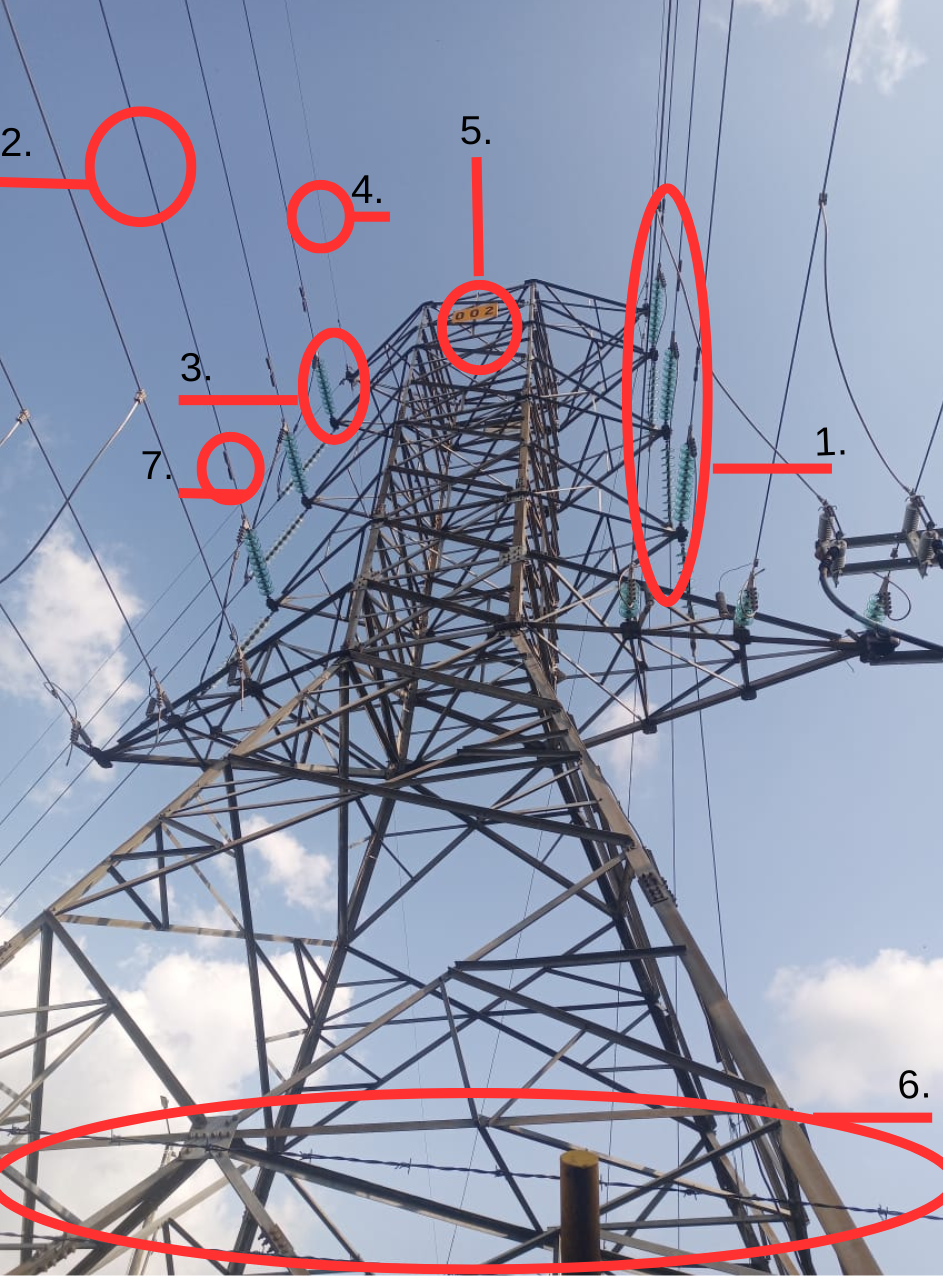
\includegraphics[width=1\textwidth]{1mer avance foticos/Torre.png}
        \caption{Torre 002 de la subestación ESSA en Floridablanca.} % Título de la figura
        \label{fig:Torre} % Etiqueta para referencias
    \end{subfigure}
    \hfill % Espacio horizontal entre las subfiguras
    \begin{subfigure}{0.5\textwidth}
        \centering % Centra la imagen
        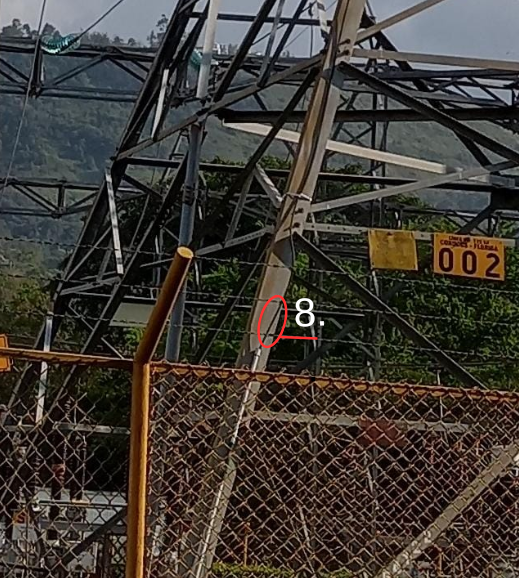
\includegraphics[width=1\textwidth]{1mer avance foticos/Torre-8.png}
        \caption{Cable de puesta a tierra de la torre 002 de la subestación ESSA en Floridablanca.} % Título de la figura
        \label{fig:Torre-8} % Etiqueta para referencias
    \end{subfigure}
\end{figure}


\end{itemize}




\section{Dimensiones y Distancias de Aislamiento}

Las principales dimensiones y distancias de aislamiento de la estructura son las siguientes:

\begin{itemize}
    \item Distancia mínima de servidumbre: 20 m.
    \item Distancia entre fases: Aproximadamente 2 m.
    \item Distancia al suelo: Aproximadamente 7 m, cumpliendo con los requisitos del RETIE.
    \item Longitud de las cadenas de aisladores: 2 m.
    

        \begin{figure}{h!}
            \centering
            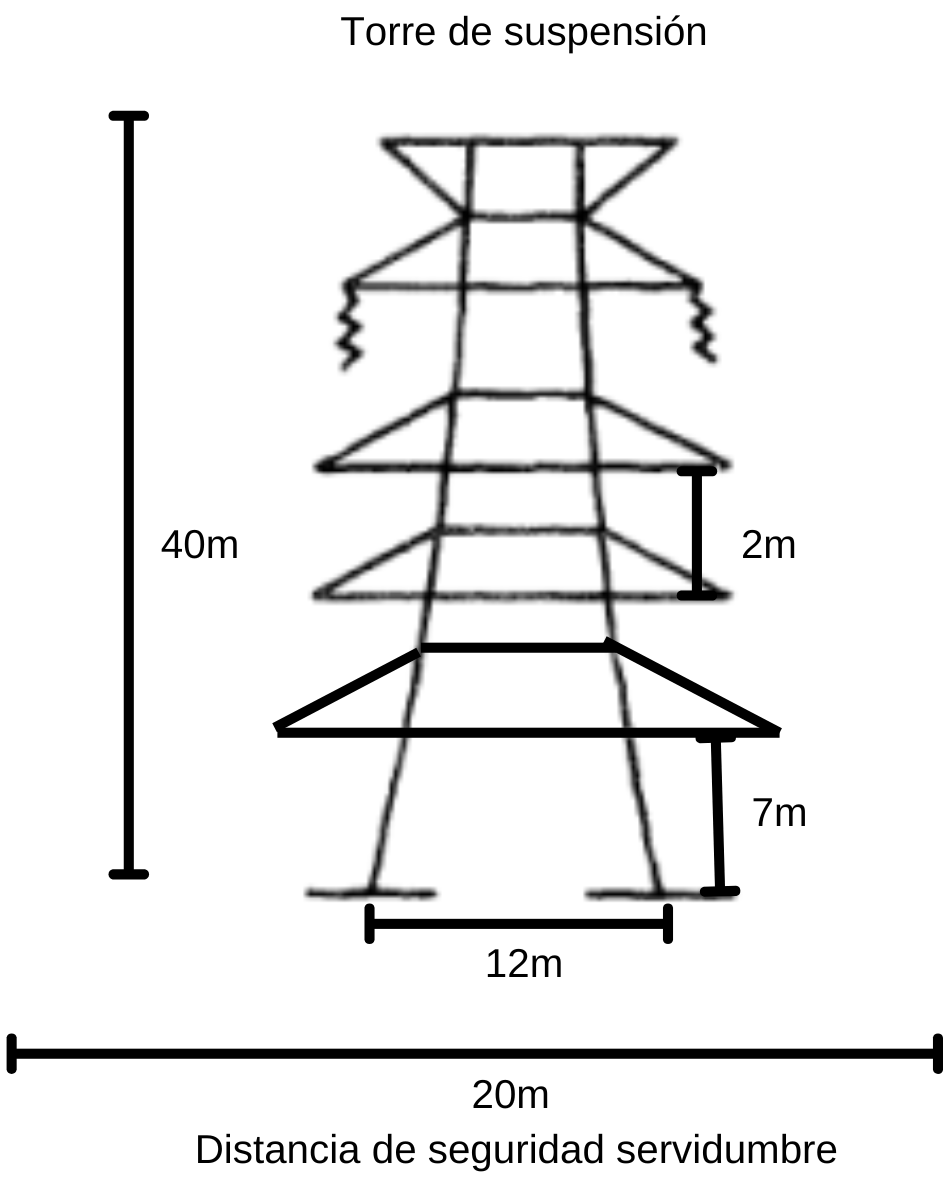
\includegraphics[width=0.5\textwidth]{1mer avance foticos/Dibujo Torre.png}
            \caption{Silueta torre 002 de la subestación ESSA en Floridablanca.} % Título de la figura
            \label{fig:Torre-Dibujo} % Etiqueta para referencias
        \end{figure}
    

\end{itemize}



\section{Cumplimiento con el RETIE}

Basándonos en la observación y sin realizar mediciones directas, se pueden analizar algunos requisitos del Reglamento Técnico de Instalaciones Eléctricas (RETIE):

\begin{itemize}
    \item \textbf{Distancia de seguridad al suelo:} La separación observada parece cumplir con la normativa, que establece un mínimo de 7 metros en zonas de tránsito restringido.
    \item \textbf{Aisladores y distancias de seguridad:} La longitud de los aisladores y la separación entre fases parecen adecuadas para evitar descargas disruptivas.
    \item \textbf{Sistema de puesta a tierra:} La presencia del cable de guarda sugiere que la torre cuenta con un sistema de protección contra sobretensiones.
    \item \textbf{Identificación y seguridad:} La existencia de una placa de identificación y un dispositivo antiescalamiento indica que la estructura cumple con los requisitos de señalización y seguridad establecidos en el RETIE.
\end{itemize}
